\iffalse
  \documentclass[mathserif, aspectratio=1610]{intbeamer}
\else
  \documentclass[aspectratio=1610]{beamer}
  \definecolor{urllinkcol}{RGB}{31,119,180}
  \hypersetup{colorlinks,linkcolor=,urlcolor=urllinkcol}
  \usetheme{Madrid}
  \usecolortheme{dove}  % dove, whale
  \usefonttheme{professionalfonts}
  \setbeamertemplate{page number in head/foot}[appendixframenumber] % appendix pagenumbering restart
\fi

\usepackage{fourier}
\usepackage[utf8]{inputenc}
\usepackage[english]{babel}
\usepackage{subcaption}
\captionsetup[subfigure]{skip=2pt} % global setting for subfigure
\usepackage{amsmath,amssymb,amsfonts}
\usepackage{bm}
\usepackage{nicefrac}
\usepackage{trfsigns}
%\usepackage{gensymb}
%\usepackage{macros}
\usepackage{xcolor}
%\usepackage{enumerate}
\setbeamercovered{invisible}
%\usepackage{tikz}
%\usetikzlibrary{calc}
\usepackage{comment}
\usepackage{drawmatrix}

%\includecomment{plottikz}
%\excludecomment{plottikz}
%\definecolor{pyplotC0}{RGB}{31,119,180}
\definecolor{C0}{HTML}{1f77b4}  % column space
\definecolor{C1}{HTML}{ff7f0e}  % left null space
\definecolor{C2}{HTML}{2ca02c}  % row space
\definecolor{C3}{HTML}{d62728}
\definecolor{C4}{HTML}{9467bd}  % null space
\definecolor{C5}{HTML}{8c564b}
\definecolor{C6}{HTML}{e377c2}
\definecolor{C7}{HTML}{7f7f7f}
\definecolor{C8}{HTML}{bcbd22}
\definecolor{C9}{HTML}{17becf}



%\newcommand{\tw}{0.73}

% ===== titlepage info =====
\title[DDASP \#24512 - Tutorial]%
{Selected Topics in Audio Signal Processing (Data-Driven Methods in Signal Processing) \#24512}

\author[Schultz, Spors]{%
    \underline{\href{https://orcid.org/0000-0002-3010-0294}{Frank Schultz}}, \href{https://orcid.org/0000-0001-7225-9992}{Sascha Spors}}

\date[Winter Term 2023/24]{%\raisebox{0mm}{\includegraphics[width=4.6cm]{logo.png}}\\
  Exercise -- Winter Term 2023/24}

\institute[]{Research Group Signal Processing and Virtual Acoustics\\
Institute of Communications Engineering\\
Faculty of Computer Science and Electrical Engineering\\
University of Rostock, Rostock, Germany}

\begin{document}
\maketitle
%
%
%
\input{orga}
%
%
%

\begin{frame}{Topics Proposal for Tutorial}
\begin{itemize}
\item singular value decomposition (SVD)
  \begin{itemize}
  \item 4 subspaces of a matrix
  \item left inverse, (right inverse)
  \item projection matrices
  \item dimensionality reduction of a feature space via PCA
  \end{itemize}
\item loss functions, empirical risk functions and numerical minimization, quality measures
\begin{itemize}
\item mean squared error for prediction
\item for binary, multinomial classification
\item gradient descent to find (a suitable) minimum
\item F-score, Rsquared, Goodness-Of-Fit Test
\end{itemize}
\item prediction models based on regression
    \begin{itemize}
    \item ordinary least squares (OLS)
    \item ridge regression
    \item SVD regression
    \end{itemize}
\item classifying models based on neural networks (NN)
  \begin{itemize}
  \item using fully connected layers (DNN)
  \item using convolutional layers (CNN)
  \end{itemize}
\end{itemize}
\end{frame}
% sketch of fields that contribute to data processing / data science
%
%
%
\begin{frame}{Literature}
  check textbooks in our main library
  \begin{itemize}
    \item \href{https://find.ub.uni-rostock.de/sk830}{SK830...SK840 statistics, (generalized) linear models, regression}
    \item ST 285...ST 306 machine learning, artifical intelligence, neural networks
    \item QH 212...QH 236 statistics mainly for economy, (generalized) linear models, regression
  \end{itemize}
  textbooks that I like very much
  \begin{itemize}
    \item Kevin P. Murphy (2022): "Probabilistic Machine Learning: An Introduction", MIT Press, 1st. ed.
    \href{https://probml.github.io/pml-book/book1.html}{current draft as free pdf}
    \item \href{https://math.mit.edu/~gs/}{Gilbert Strang} (2019): "Linear Algebra and Learning from Data", Wellesley, 1st ed.
  \end{itemize}
\end{frame}

\begin{frame}{Literature}
  theory textbooks that inspired me a lot
  \begin{itemize}
    \item S. Theodoridis, Machine Learning, 2nd ed. Academic Press, 2020.
    \href{https://www.sciencedirect.com/book/9780128188033/machine-learning}{free ebook}
    \item T. Hastie, R. Tibshirani, and J. Friedman, The Elements of Statistical Learning, 2nd ed. Springer, 2009.
    \href{https://hastie.su.domains/ElemStatLearn/}{free ebook}
    \item G. James, D. Witten, T. Hastie, and R. Tibshirani, An Introduction to Statistical Learning with Applications in R, 2nd ed. Springer, 2021. \href{https://www.statlearning.com/}{free ebook}
    \item I. Goodfellow, Y. Bengio, and A. Courville, Deep Learning. MIT Press, 2016.
    \item C.C. Aggarwal, Neural Networks and Deep Learning. Springer, 2018.
    \item C.C. Aggarwal, Linear Algebra and Optimization for Machine Learning. Springer, 2020. \href{https://link.springer.com/book/10.1007/978-3-030-40344-7}{free ebook}
    \item Marc P. Deisenroth, A. Aldo Faisal, Cheng S. Ong, Mathematics for Machine Learning, Cambridge, 2020. \href{https://mml-book.github.io/book/mml-book.pdf}{free ebook}
    \item Steven L. Brunton, J. Nathan Kutz, Data Driven Science \& Engineering, Cambridge, 2019. \href{http://www.databookuw.com/databook.pdf}{free ebook draft}
  \end{itemize}
\end{frame}

\begin{frame}{Resources}
  highly recommended web resources
  \begin{itemize}
    \item MIT course 18065 \href{https://ocw.mit.edu/courses/18-065-matrix-methods-in-data-analysis-signal-processing-and-machine-learning-spring-2018/}{Matrix Methods in Data Analysis, Signal Processing, and Machine Learning} by Gilbert Strang
    \item Steven L. Brunton, J. Nathan Kutz, Data Driven Science \& Engineering, Cambridge, 2019.
    \href{http://www.databookuw.com/databook.pdf}{free ebook draft},
    \href{http://www.databookuw.com/}{video lectures},
    \href{https://github.com/dylewsky/Data_Driven_Science_Python_Demos}{Python tutorials}
    \item A. G\'{e}ron, Hands-On Machine Learning with SciKit \& TensorFlow, 1st/2nd ed. O'Reilly, 2017/2019.
    \href{https://github.com/ageron/handson-ml2}{Python tutorials}
    \item \href{https://playground.tensorflow.org}{A Neural Network Playground---TensorFlow}
    \item courses by Andrew Ng at \url{https://www.deeplearning.ai/} and/or \url{https://www.coursera.org/}
  \end{itemize}
\end{frame}

\begin{frame}{Textbooks on Statistics}
    ML deals with stuff that is actually known for decades (at least the linear modeling part), so if we are really
    serious about to learn it deeply, we should think over concepts on
    statistical signal processing, maximum-likelihood, Bayesian vs. frequentist
    statistics, generalized linear models, hierarchical models ... ...

    textbooks that I like very much
  \begin{itemize}
  \item L. Fahrmeir, A. Hamerle, and G. Tutz, Multivariate statistische Verfahren, 2nd ed. de Gruyter, 1996.
  \href{https://www.degruyter.com/document/doi/10.1515/9783110816020/html}{free ebook}
  \item L. Fahrmeir, T. Kneib, S. Lang, and B. D. Marx, Regression, 2nd ed. Springer, 2021.
  \item A. J. Dobson and A. G. Barnett, An Introduction to Generalized Linear Models, 4th ed. CRC Press, 2018.
  \item H. Madsen, P. Thyregod, Introduction to General and Generalized Linear Models, CRC Press, 2011.
  \item A. Agresti, Foundations of Linear and Generalized Models, Wiley, 2015.
  \end{itemize}
\end{frame}





\section{Ex01: Introduction}
\begin{frame}{Ex01: Introduction}
Objectives
\begin{itemize}
\item related fields for data science / learning from data
\item model concept, un- \& supervised learning, prediction
\item idea of model parameters and hyper parameters
\item structured workflow for proper data learning
\item audio toy example that is used for linear regression and SVD demo
\end{itemize}
\end{frame}

\begin{frame}{Structured Development of Data-Driven Methods}
\textbf{Established Procedure}
\begin{enumerate}
\item Definition of the problem and of performance measures
\item Data preparation and feature extraction
\item Spot check potential model architectures
\item Model selection
\item Evaluation and reporting
\item Application
\end{enumerate}
\textbf{Technical Aspects}
\begin{itemize}
\item identify independent / dependent variables, prepare them
\item check for potential error measures and quality measures
\item choose model type(s), identify potential model parameters and hyper parameters
\item proper data handling with train/validate/test data sets
\item train/fit model(s) including optimized hyper parameters
\item choose best model(s), final train, final test, report quality
\end{itemize}
% sketch and explain x->model->y on blackboard
\end{frame}


\begin{frame}{We Can Do Machine Learning with a Linear Model}
linear algebra\footnote{we should do ourselves a favour and read at least one of the linear algebra textbooks by Gilbert Strang}
is THE tool to model linear models
\begin{center}
$
\def\Mic{3}
\def\LS{1}
\drawmatrix[fill=none, height=\Mic, width=0]y_\mathtt{M \times 1} =
\drawmatrix[fill=none, height=\Mic, width=\LS]F_\mathtt{M \times N}
\drawmatrix[fill=none, height=\LS, width=0]\theta_\mathtt{M \times 1} +
\drawmatrix[fill=none, height=\Mic, width=0]n_\mathtt{M \times 1}
$
\end{center}
\vspace{5mm}
\begin{equation*}
\bm{y} = \bm{F} \,\,\, \bm{\theta} + \bm{n}
\end{equation*}

$\bm{y}$ output data

$\bm{F}$ features as columns in a feature matrix

$\bm{\theta}$ model parameters (which we want to learn)

$\bm{n}$ noise (included in the measured output data)

\end{frame}


\begin{frame}{Audio Toy Example for Linear Regression and SVD}
Consider the following linear combinations
$$\bm{X} \bm{\beta} + \bm{n} = \bm{y}\qquad
\bm{X} \bm{\theta} + \bm{n} = \bm{y}\qquad
\bm{X} \bm{w} + \bm{n} = \bm{y}$$
where $\bm{\beta}=\bm{\theta} = \bm{w}$ are typical variables for the model parameter vector. Let us use $\bm{\beta}=[\beta_0, \beta_1, \beta_2, ..., \beta_{N-1}]^\mathrm{T}$ here, the lecture will rather utilize $\bm{\theta}$.
%
\begin{itemize}
\item $\bm{X}_{M \times N}$ matrix with $M$ audio samples for each column, $n$-th column represents the $n$-th audiotrack
\item $\bm{\beta}_{N \times 1}$ column vector of scalar values that represent a dedicated gain for each audiotrack
\item $\bm{n}_{M \times 1}$ column vector that represents a $M$-sample long noise signal added to the mixdown $\bm{X} \bm{\beta}$
\item $\bm{y}_{M \times 1}$ audio signal with $M$ samples as a result of the linear combination plus noise
\end{itemize}
%
Let us assume that i) we know $\bm{X}$ (i.e. the individual audio tracks) and $\bm{y}$ (i.e. the noise-corrupted final mixdown), ii) that we do not know the noise $\bm{n}$ and iii) that we want to estimate the 'real world' mixing gains $\bm{\theta}$
% sketch Xb=y
\end{frame}


\section{Ex02: SVD / 4 Subspaces}

\begin{frame}{Ex02: SVD / 4 Subspaces}
Objectives
\begin{itemize}
\item important matrix factorizations
\item SVD and 4 subspaces within orthonormal bases V, U
\item rank-1 matrix superposition
\end{itemize}
\end{frame}



\begin{frame}{Matrix Factorization from Eigenwert Problem for Square Matrix}

for square matrix $\bm{A}_{M \times M}$ we can have a factorization (known as diagonalization)

$$\bm{A} = \bm{X} \bm{\Lambda} \bm{X}^{-1}$$

(but only) when $M$ independent eigenvectors as columns in $\bm{X}$ (only then $\bm{X}^{-1}$ is possible)

with the corresponding eigenvalues $\lambda$ in the diagonal matrix $\Lambda$

\begin{center}
$
\def\M{1}
\def\N{1}
\def\rank{0.9999}
\drawmatrix[fill=none, height=\M, width=\N]A_\mathtt{M \times M} =
\drawmatrix[bbox style={fill=C4}, bbox height=\M, bbox width=\M, fill=C0, height=\M, width=\rank\N]X_\mathtt{M \times M}
\drawmatrix[diag]\Lambda_\mathtt{M \times M}
\drawmatrix[bbox style={fill=C4}, bbox height=\N, bbox width=\N, fill=C0, height=\N, width=\rank\N]{X}_\mathtt{M \times M}^{-1}
$
\end{center}

the matrix is acting onto $m$-th eigenvector as

$$\bm{A} \bm{x}_m = \lambda_m \bm{x}_m$$

$\Lambda$ might be complex-valued

$\bm{X}$ might be complex-valued

if some $\lambda_m=0$, we know that for this eigenvector we get $\bm{A} \bm{x}_m = 0 \bm{x}_m = \bm{0}$, i.e. $\bm{A}$ is a singular matrix, i.e. $\bm{A}$ is a non-full rank matrix

\end{frame}




\begin{frame}{Matrix Factorization from Eigenwert Problem for Symmetric Matrix}

for \underline{symmetric} matrix $\bm{A}_{M \times M} = \bm{A}_{M \times M}^H$ we can have a special case of diagonalization

$$\bm{A} = \bm{Q} \bm{\Lambda} \bm{Q}^{-1} = \bm{Q} \bm{\Lambda} \bm{Q}^{H}$$

(only) when $M$ independent, \underline{orthogonal} eigenvectors as columns in $\bm{Q}$ \quad($\bm{Q} \bm{Q}^H = \bm{I}$, $\bm{Q}^H \bm{Q} = \bm{I}$)

with the corresponding eigenvalues $\lambda\in\mathbb{R}$ in the diagonal matrix $\Lambda$

\begin{center}
$
\def\M{1}
\def\N{1}
\def\rank{0.9999}
\drawmatrix[fill=none, height=\M, width=\N]A_\mathtt{M \times M} =
\drawmatrix[bbox style={fill=C4}, bbox height=\M, bbox width=\M, fill=C1, height=\M, width=\rank\N]{Q}_\mathtt{M \times M}
\drawmatrix[diag]\Lambda_\mathtt{M \times M}
\drawmatrix[bbox style={fill=C4}, bbox height=\N, bbox width=\N, fill=C1, height=\N, width=\rank\N]{Q}_\mathtt{M \times M}^{H}
$
\end{center}

the matrix is acting onto $m$-th eigenvector as

$$\bm{A} \bm{q}_m = \lambda_m \bm{q}_m$$

$\Lambda\in\mathbb{R}$

$\bm{Q}\in\mathbb{R}$ if $\bm{A}\in\mathbb{R}$, $\bm{Q}\in\mathbb{C}$ if $\bm{A}\in\mathbb{C}$

if some $\lambda_m=0$ we know that for this eigenvector we get $\bm{A} \bm{q}_m = 0 \bm{q}_m = \bm{0}$, i.e. $\bm{A}$ is a singular matrix, i.e. $\bm{A}$ is a non-full rank matrix
\end{frame}







\begin{frame}{Generalized Factorization?!?}
Over-Determined
\begin{center}
$
\def\M{3}
\def\N{1}
\def\rank{0.8}
\drawmatrix[fill=none, height=\M, width=\N]A_\mathtt{M \times N} =
\drawmatrix[bbox style={fill=C4}, bbox height=\M, bbox width=\M, fill=C0, height=\M, width=\rank\N]U_\mathtt{M \times M}
\drawmatrix[bbox style={fill=gray!50}, bbox height=\M, bbox width=\N, fill=white, height=\rank\N, width=\rank\N]\Sigma_\mathtt{M \times N}
\drawmatrix[bbox style={fill=C1}, bbox height=\N, bbox width=\N, fill=C2, height=\N, width=\rank\N]{V}_\mathtt{N \times N}^H
$
\end{center}
Under-Determined
\begin{center}
$
\def\M{1}
\def\N{3}
\def\rank{0.2}
\drawmatrix[fill=none, height=\M, width=\N]A_\mathtt{M \times N} =
\drawmatrix[bbox style={fill=C4}, bbox height=\M, bbox width=\M, fill=C0, height=\M, width=\rank\M]U_\mathtt{M \times M}
\drawmatrix[bbox style={fill=gray!50}, bbox height=\M, bbox width=\N, fill=white, height=\rank\M, width=\rank\M]\Sigma_\mathtt{M \times N}
\drawmatrix[bbox style={fill=C1}, bbox height=\N, bbox width=\N, fill=C2, height=\N, width=\rank\M]{V}_\mathtt{N \times N}^H
$
\end{center}
\end{frame}



\begin{frame}{Singular Value Decomposition (SVD)}
most general matrix factorization % that nicely reveals the 4 subspaces of a rank $r$ matrix $\bm{A}$

fundamentally important for understanding the heart beat of linear algebra

\begin{center}
$
\def\M{2}
\def\N{1}
\def\rank{0.999999}
\drawmatrix[fill=none, height=\M, width=\N]A_\mathtt{M \times N} =
\drawmatrix[bbox style={fill=C4}, bbox height=\M, bbox width=\M, fill=C0, height=\M, width=\rank\N]U_\mathtt{M \times M}
\drawmatrix[bbox style={fill=gray!50}, bbox height=\M, bbox width=\N, fill=white, height=\rank\N, width=\rank\N]\Sigma_\mathtt{M \times N}
\drawmatrix[bbox style={fill=C1}, bbox height=\N, bbox width=\N, fill=C2, height=\N, width=\rank\N]{V}_\mathtt{N \times N}^H
$
\end{center}

\begin{center}
$
\def\M{1}
\def\N{2}
\def\rank{0.999999}
\drawmatrix[fill=none, height=\M, width=\N]A_\mathtt{M \times N} =
\drawmatrix[bbox style={fill=C4}, bbox height=\M, bbox width=\M, fill=C0, height=\M, width=\rank\M]U_\mathtt{M \times M}
\drawmatrix[bbox style={fill=gray!50}, bbox height=\M, bbox width=\N, fill=white, height=\rank\M, width=\rank\M]\Sigma_\mathtt{M \times N}
\drawmatrix[bbox style={fill=C1}, bbox height=\N, bbox width=\N, fill=C2, height=\N, width=\rank\M]{V}_\mathtt{N \times N}^H
$
\end{center}

$$\bm{A} = \bm{U} \bm{\Sigma} \bm{V}^\mathrm{H}$$


left singular vectors\quad$\bm{U} = \mathrm{eigvec}(\bm{A}\bm{A}^\mathrm{H})$
\begin{footnotesize}, order must match to the corresponding singular values\end{footnotesize}

right singular vectors $\bm{V} = \mathrm{eigvec}(\bm{A}^\mathrm{H}\bm{A})$
\begin{footnotesize}, order must match to the corresponding singular values\end{footnotesize}

singular value matrix $\bm{\Sigma}$, $r$ singular values on \underline{diagonal} descending order

\end{frame}


\begin{frame}{Singular Value Decomposition (SVD)}
input-related matrix $\bm{V}$ and output related matrix $\bm{U}$ are unitary, i.e.

$$\bm{V}\bm{V}^\mathrm{H}=\bm{I},\quad\bm{V}^\mathrm{H}\bm{V}=\bm{I},\quad\bm{U}\bm{U}^\mathrm{H}=\bm{I},\quad\bm{U}^\mathrm{H}\bm{U}=\bm{I}$$

superposition of rank-1 matrices (outer products) because singular values in diagonal matrix $\bm{\Sigma}$
$$\bm{A} = \sum_{i=1}^{\text{rank }r} \sigma_i \bm{u}_i \bm{v}_i^\mathrm{H} = \bm{U} \bm{S} \bm{V}^\mathrm{H}$$

Fundamentally important: $\bm{U}$ and $\bm{V}$ span the 4 subspaces of matrix $\bm{A}$

\centering
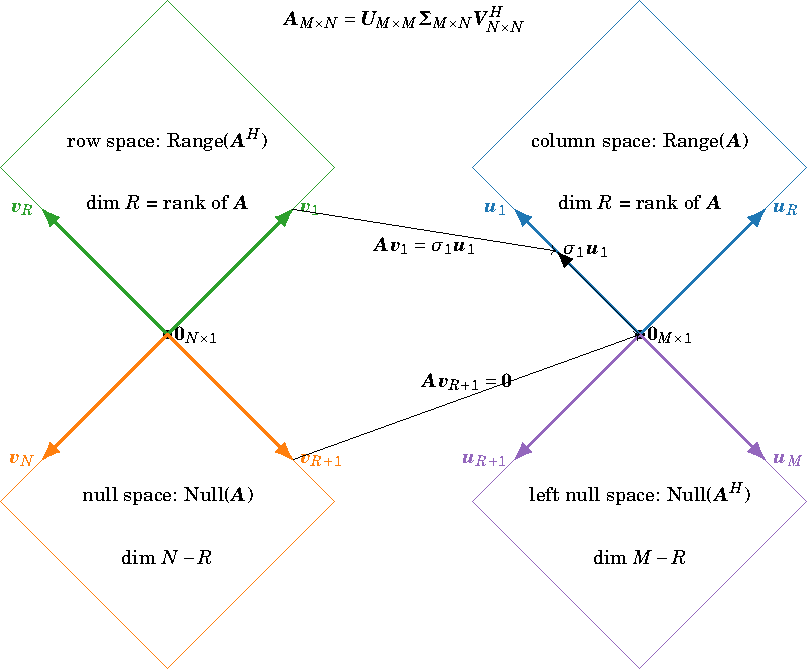
\includegraphics[width=0.4\textwidth]{four_subspaces.pdf}

\end{frame}

\begin{frame}{The 4 Subspaces of a Matrix}

matrix $\bm{A}_{M \times N} = \bm{U} \bm{\Sigma} \bm{V}^H$ spans four fundamental subspaces

\hspace{4.25cm}
\textcolor{C0}{column space} $\perp$ \textcolor{C4}{left null space}
\hspace{0.75cm}
\textcolor{C2}{row space} $\perp$ \textcolor{C1}{null space}

\textcolor{C0}{column space / range / image:} $$R(\bm{A}) = \{\bm{p}\in\mathbb{C}^M | \bm{A} \bm{g} = \bm{p},\qquad\forall \bm{g}\in\mathbb{C}^N\}$$

\textcolor{C1}{null space / kernel:} $$N(\bm{A}) = \{\bm{g}\in\mathbb{C}^N | \bm{A} \bm{g} = \bm{0}\}$$

the column/null-space concept for transposed matrix $\bm{A}^H$ yields the two other spaces:

\textcolor{C2}{row space:} $$R(\bm{A}^H) = \{\bm{g}\in\mathbb{C}^N | \bm{A}^H \bm{p} = \bm{g},\qquad\forall \bm{p}\in\mathbb{C}^M\}$$

\textcolor{C4}{left null space / cokernel:} $$N(\bm{A}^H) = \{\bm{p}\in\mathbb{C}^M | \bm{A}^H \bm{p} = \bm{0}\}$$

rank of $\bm{A}$ == dimension of column space == dimension of row space == number of independent columns and rows

\end{frame}
%
%
%
\begin{frame}{4 Subspaces of a Matrix}

matrix $\bm{A}_{M \times N} = \bm{U} \bm{\Sigma} \bm{V}^H$ spans four fundamental subspaces, these are nicely encoded in the SVD

\hspace{0.75cm}
\textcolor{C2}{row space} $\perp$ \textcolor{C1}{null space}
\hspace{4.5cm}
\textcolor{C0}{column space} $\perp$ \textcolor{C4}{left null space}

\centering
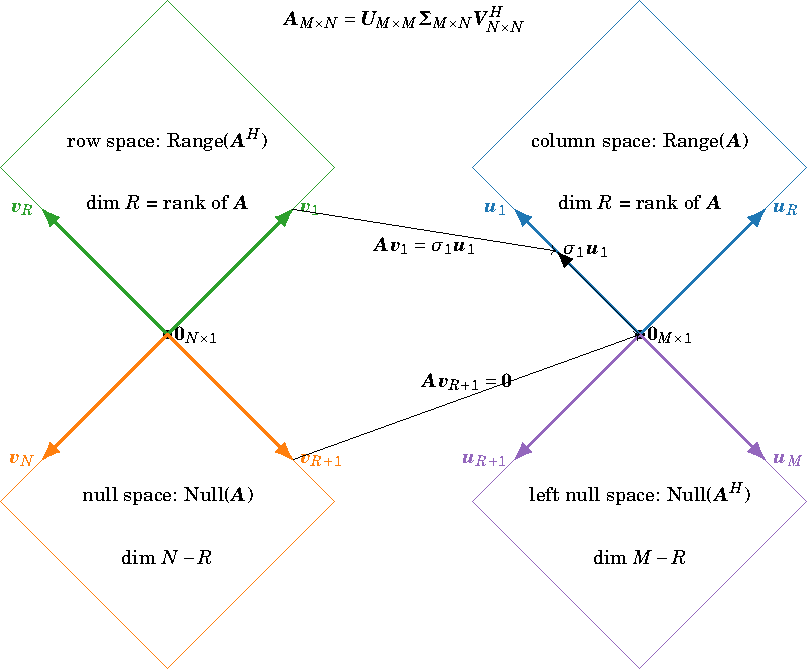
\includegraphics[width=0.5\textwidth]{four_subspaces.pdf}

\hspace{0.75cm}
right singular vectors in $\bm{V}$
\hspace{4.5cm}
left singular vectors in $\bm{U}$

\end{frame}
%
%
%
\begin{frame}{Singular Value Decomposition (SVD), full rank cases}

$\cdot$ Sum of rank-1 matrices\qquad
$\bm{A} = \bm{U} \bm{\Sigma} \bm{V}^H =  \sum\limits_{i=1}^{r} \sigma_i \quad \textcolor{C0}{\bm{u}}_i \quad \textcolor{C2}{\bm{v}}^H_i$

\hspace{4.25cm}
\textcolor{C0}{column space} $\perp$ \textcolor{C4}{left null space}
\hspace{0.75cm}
\textcolor{C2}{row space} $\perp$ \textcolor{C1}{null space}

$\cdot$ Square matrix $\bm{A}$, \quad $M$ rows $=$ $N$ columns, \quad full rank ($r=M=N$), \quad inverse $\bm{A}^\dagger = \bm{A}^{-1}$
\begin{center}
$
\def\M{1}
\def\N{1}
\def\rank{0.999999}
\drawmatrix[fill=none, height=\M, width=\N]A_\mathtt{M \times N} =
\drawmatrix[bbox style={fill=C4}, bbox height=\M, bbox width=\M, fill=C0, height=\M, width=\rank\N]U_\mathtt{M \times M}
\drawmatrix[bbox style={fill=gray!50}, bbox height=\M, bbox width=\N, fill=white, height=\rank\N, width=\rank\N]\Sigma_\mathtt{M \times N}
\drawmatrix[bbox style={fill=C1}, bbox height=\N, bbox width=\N, fill=C2, height=\N, width=\rank\N]{V}_\mathtt{N \times N}^H
$
\end{center}
$\cdot$ Flat / fat matrix $\bm{A}$, \quad $M$ rows $<$ $N$ columns, \quad full row rank ($r=M$), \quad right inverse $\bm{A}^\dagger = \bm{A}^H (\bm{A} \bm{A}^H )^{-1}$
\begin{center}
$
\def\M{1}
\def\N{1.4}
\def\rank{0.999999}
\drawmatrix[fill=none, height=\M, width=\N]A_\mathtt{M \times N} =
\drawmatrix[bbox style={fill=C4}, bbox height=\M, bbox width=\M, fill=C0, height=\M, width=\rank\M]U_\mathtt{M \times M}
\drawmatrix[bbox style={fill=gray!50}, bbox height=\M, bbox width=\N, fill=white, height=\rank\M, width=\rank\M]\Sigma_\mathtt{M \times N}
\drawmatrix[bbox style={fill=C1}, bbox height=\N, bbox width=\N, fill=C2, height=\N, width=\rank\M]{V}_\mathtt{N \times N}^H
$
\end{center}
$\cdot$ Tall / thin matrix $\bm{A}$, \quad $M$ rows $>$ $N$ columns, \quad full column rank ($r=N$), \quad left inverse $\bm{A}^\dagger = (\bm{A}^H \bm{A})^{-1} \bm{A}^H$
\begin{center}
$
\def\M{1.4}
\def\N{1}
\def\rank{0.999999}
\drawmatrix[fill=none, height=\M, width=\N]A_\mathtt{M \times N} =
\drawmatrix[bbox style={fill=C4}, bbox height=\M, bbox width=\M, fill=C0, height=\M, width=\rank\N]U_\mathtt{M \times M}
\drawmatrix[bbox style={fill=gray!50}, bbox height=\M, bbox width=\N, fill=white, height=\rank\N, width=\rank\N]\Sigma_\mathtt{M \times N}
\drawmatrix[bbox style={fill=C1}, bbox height=\N, bbox width=\N, fill=C2, height=\N, width=\rank\N]{V}_\mathtt{N \times N}^H
$
\end{center}
\end{frame}
%
%
%
\begin{frame}{Singular Value Decomposition (SVD), rank-deficient cases}

$\cdot$ Sum of rank-1 matrices\qquad
$\bm{A} = \bm{U} \bm{\Sigma} \bm{V}^H =  \sum\limits_{i=1}^{r} \sigma_i \quad \textcolor{C0}{\bm{u}}_i \quad \textcolor{C2}{\bm{v}}^H_i$

\hspace{4.25cm}
\textcolor{C0}{column space} $\perp$ \textcolor{C4}{left null space}
\hspace{0.75cm}
\textcolor{C2}{row space} $\perp$ \textcolor{C1}{null space}

$\cdot$ Square matrix $\bm{A}$, \quad $M$ rows $=$ $N$ columns, \quad rank deficient ($r<M=N$), \quad pseudo-inverse $\bm{A}^\dagger = \bm{V} \Sigma^\dagger \bm{U}^H$
\begin{center}
$
\def\M{1}
\def\N{1}
\def\rank{0.5}
\drawmatrix[fill=none, height=\M, width=\N]A_\mathtt{M \times N} =
\drawmatrix[bbox style={fill=C4}, bbox height=\M, bbox width=\M, fill=C0, height=\M, width=\rank\N]U_\mathtt{M \times M}
\drawmatrix[bbox style={fill=gray!50}, bbox height=\M, bbox width=\N, fill=white, height=\rank\N, width=\rank\N]\Sigma_\mathtt{M \times N}
\drawmatrix[bbox style={fill=C1}, bbox height=\N, bbox width=\N, fill=C2, height=\N, width=\rank\N]{V}_\mathtt{N \times N}^H
$
\end{center}
$\cdot$ Flat / fat matrix $\bm{A}$, \quad $M$ rows $<$ $N$ columns, \quad rank deficient ($r<M$), \quad pseudo-inverse $\bm{A}^\dagger = \bm{V} \Sigma^\dagger \bm{U}^H$
\begin{center}
$
\def\M{1}
\def\N{1.4}
\def\rank{0.75}
\drawmatrix[fill=none, height=\M, width=\N]A_\mathtt{M \times N} =
\drawmatrix[bbox style={fill=C4}, bbox height=\M, bbox width=\M, fill=C0, height=\M, width=\rank\M]U_\mathtt{M \times M}
\drawmatrix[bbox style={fill=gray!50}, bbox height=\M, bbox width=\N, fill=white, height=\rank\M, width=\rank\M]\Sigma_\mathtt{M \times N}
\drawmatrix[bbox style={fill=C1}, bbox height=\N, bbox width=\N, fill=C2, height=\N, width=\rank\M]{V}_\mathtt{N \times N}^H
$
\end{center}
$\cdot$ Tall / thin matrix $\bm{A}$, \quad $M$ rows $>$ $N$ columns, \quad rank deficient ($r<N$), \quad pseudo-inverse $\bm{A}^\dagger = \bm{V} \Sigma^\dagger \bm{U}^H$
\begin{center}
$
\def\M{1.4}
\def\N{1}
\def\rank{0.67}
\drawmatrix[fill=none, height=\M, width=\N]A_\mathtt{M \times N} =
\drawmatrix[bbox style={fill=C4}, bbox height=\M, bbox width=\M, fill=C0, height=\M, width=\rank\N]U_\mathtt{M \times M}
\drawmatrix[bbox style={fill=gray!50}, bbox height=\M, bbox width=\N, fill=white, height=\rank\N, width=\rank\N]\Sigma_\mathtt{M \times N}
\drawmatrix[bbox style={fill=C1}, bbox height=\N, bbox width=\N, fill=C2, height=\N, width=\rank\N]{V}_\mathtt{N \times N}^H
$
\end{center}
\end{frame}

\begin{frame}{Subspace Properties and Characteristics of Inverse Problem}
%
sketches of the 4 subspaces for these 4 cases help to get the essence how a matrix maps things forward and (potentially) backward
%
\begin{itemize}
\item full rank, no nullspace, no left null space = square matrix = exactly solvable, typically learned in basic linear algebra course
\item full column rank, no nullspace, potentially large left nullspace = tall/thin matrix, over determined system of equations, we need the left inverse, many practical problems, statistical model fitting, least squares error solution
\item full row rank, potentially large nullspace, no left nullspace = flat/fat matrix, under-determined system of equations, we need the right inverse, solution in the sense of least squares magnitude for unknown vector
\item rank deficient, potentially large nullspace, potentially large left nullspace, meaningful information of the matrix is not stored in optimum way $\rightarrow$ data-driven learning...but before doing this stuff, we should at least learn full column rank cases properly
\end{itemize}
%
\end{frame}


\begin{frame}{SVD Basics}
due to $\bm{V}^\mathrm{H}\bm{V}=\bm{I}$ we can re-arrange
$$\bm{A} = \bm{U} \bm{\Sigma} \bm{V}^\mathrm{H} \rightarrow
\bm{A} \bm{V} = \bm{U} \bm{\Sigma}$$
rank $r$ matrix $\bm{A}$ acting on row space $\bm{v}$ maps to corresponding column space $\bm{u}$ weighted by corresponding singular value
$$\bm{A} \bm{v}_{1:r} = \sigma_{1:r} \bm{u}_{1:r}$$
matrix acting on null space $\bm{v}$ maps to zero vector $\bm{0}_{M \times 1}$
$$\bm{A} \bm{v}_{r+1:N} = \bm{0}$$
we should make a sketch to visualisze this

\centering
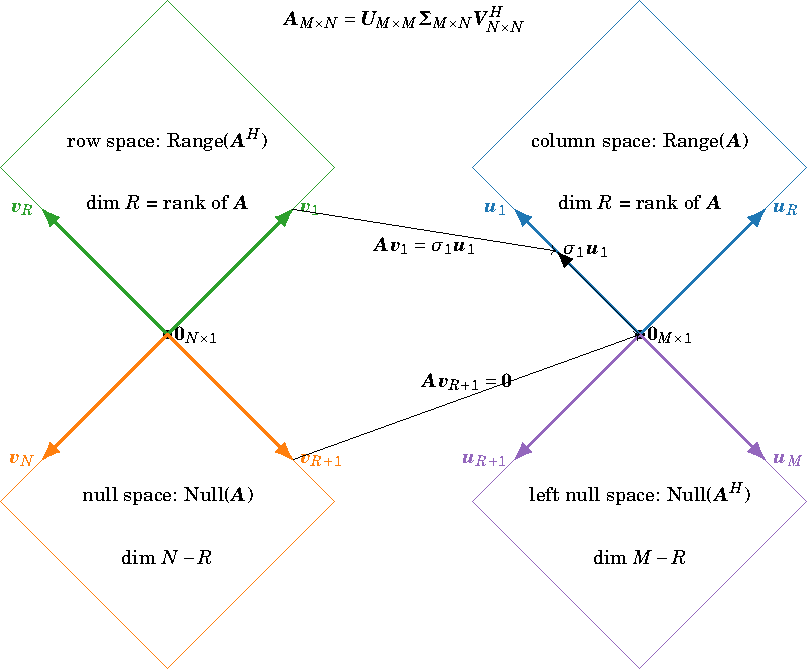
\includegraphics[width=0.3\textwidth]{four_subspaces.pdf}

\end{frame}

































\section{Ex03: SVD and Left Inverse Brings us to OLS Linear Regression}

\begin{frame}{Ex03: SVD and Left Inverse Brings us to OLS Linear Regression}
Objectives
\begin{itemize}
\item linear regression with least squares error teaser
\item subspaces example on simple matrix
\item nice SVD properties and essence
\item projecting vectors onto $\bm{U}$ and $\bm{V}$ spaces
\item for full column rank matrix $\bm{X}_{M \times N}$ we can try to bring a $\bm{y}\in \mathbb{R}^M$ back to $\bm{\beta}\in \mathbb{R}^N$ solving the inverse problem for $\bm{X} \bm{\beta} + \bm{n} = \bm{y}$...we should do this by understanding the SVD
\item we then re-invented the so called left inverse of a matrix
\item this can be used to solve an inverse problem in ordinary least squares (OLS) sense
\item we check this with geometrical considerations rather than calculus
\end{itemize}
\end{frame}







\begin{frame}{Projection into V}
\begin{itemize}
\item
tall, thin and full column rank matrix $\bm{X}_{M \times N}$ with rank $r=N$ and SVD $\bm{X} = \bm{U} \bm{S} \bm{V}^\mathrm{H}$
\item
we assume a made up vector $\bm{\beta} = 1.234 \bm{v}_1 + 5.678 \bm{v}_r$
\item
we should project $\bm{\beta}$ onto the $\bm{v}$ vectors, which needs $(\bm{v}_{1:r}^\mathrm{H} \bm{\beta}) \bm{v}_{1:r} = ?$
\item
we get $\bm{v}_{1}^\mathrm{H} \bm{\beta} = 1.234$, $\bm{v}_{2:r-1}^\mathrm{H} \bm{\beta} = 0$, $\bm{v}_{r}^\mathrm{H} \bm{\beta} = 5.678$ for the weights of the $\bm{v}$
space vectors, not suprisingly due to orthonormality of the $\bm{V}$ matrix
\item
linear combination $(\bm{v}_{1}^\mathrm{H} \bm{\beta})\bm{v}_1 + 0 + ... + 0 + (\bm{v}_{r}^\mathrm{H} \bm{\beta})\bm{v}_r = \bm{\beta}$ yields precisely the made up vector $\bm{\beta}$ that we started with
\item
a made up vector $\bm{\alpha}$ might have non-zero weights for all $\bm{v}$ vectors, i.e. all $\bm{v}$ vectors really contribute to the spanning job...
\item
we should start to think always in linear combinations of SVD's $\bm{V}$ and $\bm{U}$ spaces
\item
as always a simple sketch is helping to understand
\item
all projections at once is written as $\bm{V}^\mathrm{H} \bm{\beta}$, cf. $\bm{X}\bm{\beta} = \bm{U} \bm{S} \bm{V}^\mathrm{H}\bm{\beta}$
\end{itemize}
\end{frame}


\begin{frame}{Left Inverse Via SVD}
we want to solve for ${\bm{\beta}}$, full column rank $\bm{X}_{M \times N}$, rank $r=N$
$$\bm{X} {\bm{\beta}} = \bm{y}$$
apply SVD
$$\bm{U} \bm{S} \bm{V}^\mathrm{H} {\bm{\beta}} = \bm{y}$$
get weights of U space projection
$$\bm{U}^\mathrm{H} \bm{U} \bm{S} \bm{V}^\mathrm{H} {\bm{\beta}} = \bm{U}^\mathrm{H}\bm{y}$$
invert all singular values and setup $\bm{S}^\dagger_{N \times M} = [\mathrm{diag}(1/\sigma_i) \quad \bm{0}]$ such that
$\bm{S}^\dagger\bm{S} = \bm{I}_{N \times N}$, apply
$$\bm{S}^\dagger\bm{S} \bm{V}^\mathrm{H} {\bm{\beta}} = \bm{S}^\dagger\bm{U}^\mathrm{H}\bm{y}$$
let matrix $\bm{V}$ act on this vector, i.e. map as linear combination into row space in $\bm{V}$
$$\bm{V} \bm{V}^\mathrm{H} {\bm{\beta}} = \bm{V} \bm{S}^\dagger\bm{U}^\mathrm{H}\bm{y}
\rightarrow \text{this yields our estimator } \hat{\bm{\beta}} = \bm{V} \bm{S}^\dagger\bm{U}^\mathrm{H}\bm{y} = \bm{X}^\dagger \bm{y}$$
we might want to show that the left inverse $\bm{X}^\dagger$ can be written equivalently as
$$\bm{V} \bm{S}^\dagger\bm{U}^\mathrm{H} = (\bm{X}^\mathrm{H}\bm{X})^{-1} \bm{X}^\mathrm{H} = \bm{X}^\dagger$$
\end{frame}



\begin{frame}{Left Inverse Via SVD}
full column rank $\bm{X}_{M \times N}$, rank $r=N$, singular values $\sigma_1 > \sigma_2 > \sigma_i > \sigma_r > 0$

forward problem: map (row space+null space) to column space with $\bm{X} \bm{\beta} = \bm{y}$
$$
\bm{X}_{M \times N}
=
\bm{U}_{M \times M}\quad
\bm{S}_{M \times N}\quad
(\bm{V}_{N \times N})^\mathrm{H}=
\bm{U}
\begin{bmatrix}
\sigma_1  & 0  & 0 & 0\\
0 & \sigma_2 & 0 & 0\\
0 & 0 & \sigma_i & 0\\
0 & 0 & 0 & \sigma_r\\
0 & 0 & 0 & 0\\
0 & 0 & 0 & 0
\end{bmatrix}
\bm{V}^\mathrm{H}
$$
inverse problem: map (column space+left null space) to row space with left inverse $\bm{X}^\dagger \bm{y} = \bm{\beta}$
$$
\bm{X}^\dagger_{N \times M}
=
\bm{V}_{N \times N}\quad
\bm{S}^\dagger_{N \times M}\quad
(\bm{U}_{M \times M})^\mathrm{H}
=
\bm{V}
\begin{bmatrix}
\frac{1}{\sigma_1} & 0 & 0 & 0 & 0 & 0\\
0 & \frac{1}{\sigma_2} & 0 & 0 & 0 & 0\\
0 & 0 & \frac{1}{\sigma_i} & 0 & 0 & 0\\
0 & 0 & 0 & \frac{1}{\sigma_r} & 0 & 0\\
\end{bmatrix}
\bm{U}^\mathrm{H}
$$






\end{frame}





\begin{frame}{Projection Matrices Based on Left Inverse}
For full column rank $\bm{X}_{M \times N}$, rank $r=N$ we got the left inverse
$$\bm{V} \bm{S}^\dagger\bm{U}^\mathrm{H} = (\bm{X}^\mathrm{H}\bm{X})^{-1} \bm{X}^\mathrm{H} = \bm{X}^\dagger_{N \times M}$$
from which we can create four projection matrices into the four subspaces
\begin{itemize}
\item into row space $\bm{P}_\text{row} = \bm{X}^\dagger \bm{X} = \bm{I}_{N \times N}$ \begin{footnotesize}(i.e. the concept of a left inverse)\end{footnotesize}
\item into null space $\bm{P}_\text{null} = \bm{I} - \bm{P}_\text{row} = \bm{0}_{N \times N}$ \begin{footnotesize}(because no null space when full column rank)\end{footnotesize}
\item into column space $\bm{P}_\text{column} = (\bm{X} \bm{X}^\dagger)_{M \times M}$ \begin{footnotesize}(very often called hat matrix)\end{footnotesize}
\item into left nullspace $\bm{P}_\text{left null} = \bm{I}_{M \times M} - \bm{P}_\text{column}$
\end{itemize}

So the estimator $\hat{\bm{\beta}}$ from solving the inverse problem yields a vector living in the column space
$$\bm{X} \hat{\bm{\beta}} = \bm{X} (\bm{X}^\dagger \bm{y}) = \bm{P}_\text{column} \bm{y} = \hat{\bm{y}}$$
This means that there is a remaining part (typical called residual) $\bm{e}$ from measured $\bm{y}$
$$\bm{e} = \bm{y} - \hat{\bm{y}} = \bm{y} - \bm{P}_\text{column} \bm{y} = (\bm{I}_{M \times M} - \bm{P}_\text{column}) \bm{y}=
\bm{P}_\text{left null} \bm{y} = \bm{e}$$
which lives in the left null space. Due to the orthogonal subspaces, we know that $\hat{\bm{y}} \perp \bm{e}$

\end{frame}

\begin{frame}{Least Squares Sense Solution: Calculus vs. Graphical}
Calculus way: As usually assuming full column rank, we can consider an optimization problem, where we want to minimize
squared distance, hence the name least squares
$$\min_{\text{wrt }\bm{\beta}} ||\bm{y} - \bm{X} \bm{\beta}||_2^2$$
which needs 1st / 2nd derivatives, yielding the already found solution using the left inverse
$$\hat{\bm{\beta}} = (\bm{X}^\mathrm{H}\bm{X})^{-1} \bm{X}^\mathrm{H} \bm{y}$$
Graphical way: the shortest path to get $\bm{y}$ into the column space is by orthogonal projection, we get again $\hat{\bm{y}} \perp \bm{e}$...that's why the subspace
stuff is so nice...the $\hat{\bm{y}}$ can be mapped back to row space yielding $\hat{\bm{\beta}}$
\begin{center}
\includegraphics[width=0.23\textwidth]{figures_web/Theodoridis_ML_2nd_Fig4.3.png}
\end{center}
\begin{footnotesize}consider Fig. 4.3 from S. Theodoridis, Machine Learning, 2nd ed. Academic Press, 2020\end{footnotesize}
\end{frame}

\section{Ex04: Audio Example, Linear Regression, SVD}
\begin{frame}{Ex04: SVD Factorization of Multitrack Audio}
Objectives: understanding the essence of SVD vs. utilizing SVD on real data
%we can listen to audio or view images, so we should bring memorizable examples that feature these senses

\begin{itemize}
\item given a $M \times N$ matrix $\bm{X}$ with full column rank $r=N$ containing $M$ audio samples on $N$ channels, this might be a studio recording of a song, e.g. 1st channel is bassdrum, 2nd is bass guitar, $N$-th channel is a synth line
\item perform an economy size SVD on this multitrack audio data (a normal SVD would need way too much RAM to store left nullspace in $\bm{U}$)
$$\bm{X} = \bm{U} \bm{S} \bm{V}^\mathrm{H}$$
\item we can listen to and plot the weighted left singular vectors that span the column space
$$\mathbf{H}_{M \times r} =  \mathbf{U}_{M \times r} \mathbf{S}_{r \times r}$$
\item we could analyze polarity / level of the mixing weights $\mathbf{V}^\mathrm{H} \mathbf{g}$ of the mixdown
$$\mathbf{y} = \mathbf{X}\mathbf{g} = \mathbf{H} \cdot \mathbf{V}^\mathrm{H} \mathbf{g}$$
\item we could listen to the mixdown using the best rank $q<=r$ approximation
$$\mathbf{y} =\bm{U} \bm{S}_q \bm{V}^\mathrm{H}\mathbf{g}$$
\end{itemize}

\end{frame}

\section{Ex05: Audio Example}
\begin{frame}{Ex05: Audio Example}
Objectives
%\begin{itemize}
%\end{itemize}
\end{frame}






\section{Exxx: TBD}
\begin{frame}{Audio Toy Example for Music Genre Classification}
TBD...
\end{frame}


% \section{Ex0x: Topic}
% \begin{frame}{Ex0x: Topic}
% Objectives
% \begin{itemize}
% \item
% \end{itemize}
% \end{frame}



\appendix

\section{Appendix: SVD Example Manual Calculus}
\begin{frame}{SVD Example Manual Calculus: Problem Definition and First Expectations}
We should calculate the SVD of the simple $M \times N$ matrix
$$\bm{X} =
\begin{bmatrix}
1\\2
\end{bmatrix}
\begin{bmatrix}
1 & 3
\end{bmatrix}
=
\begin{bmatrix}
1 & 3\\
2 & 6
\end{bmatrix}
\stackrel{?}{=}
\bm{U}\bm{S}\bm{V}^\mathrm{T}
$$
manually.

Before, we start, let us realize what we have here.

The single outer product tells us immediately that we deal with a rank $r=1$ matrix, expecting dependencies
in rows and columns.

We immediately see that i) rows are dependent because row2 = 2 row1, ii) columns are dependent because col2 = 3 col1.

Due to rank $r=1$, we expect only one non-zero singular value $\sigma_1$, therefore the dimension
of row space (which is always equal to the dimension of column space) is $r=1$, i.e. we have $r$
independent vectors that span the row space and $r$ independent vectors that span the column space, so these spaces are lines in both 2D spaces in our example.

The $\bm{U}$ space has vectors in $\mathbb{R}^{M=2}$, the $\bm{V}$ space has vectors in $\mathbb{R}^{N=2}$.

\end{frame}


\begin{frame}{SVD Example Manual Calculus: Further Expectations}
$$\bm{X} =
\begin{bmatrix}
1\\2
\end{bmatrix}
\begin{bmatrix}
1 & 3
\end{bmatrix}
=
\begin{bmatrix}
1 & 3\\
2 & 6
\end{bmatrix}
$$

This simple single outer product gives us direct access to the column space, as this is a $\bm{X}=\bm{C}\bm{R}$ factorization; it is the line along the column vector
$$
\begin{bmatrix}
1\\2
\end{bmatrix}
$$
Furthermore, we directly can deduce the row space, which is the line along the
column vector
$$
\begin{bmatrix}
1\\3
\end{bmatrix},
$$
i.e. the transposed row found in the outer product. So, all $X^\mathrm{T} \bm{y}$,
except those solutions that produce $X^\mathrm{T} \bm{y} = \bm{0}$ (these $\bm{y}$
belong to the left null space), are multiples of $[1, 3]^\mathrm{T}$.


\end{frame}



\begin{frame}{SVD Example Manual Calculus: Further Expectations 2}
$$\bm{X} =
\begin{bmatrix}
1\\2
\end{bmatrix}
\begin{bmatrix}
1 & 3
\end{bmatrix}
=
\begin{bmatrix}
1 & 3\\
2 & 6
\end{bmatrix}
\stackrel{?}{=}
\bm{U}\bm{S}\bm{V}^\mathrm{T}
$$

As we have $M-r$ vectors that span the left null space, thus here $M=2$ and $r=1$,
the left nullspace is a line orthogonal to the column space (line).

As we have $N-r$ vectors that span the null space, thus here $N=2$ and $r=1$,
the nullspace is a line orthogonal to the row space (line).

We should meet these expectations, when calculating the SVD manually.

\end{frame}




\begin{frame}{SVD Example Manual Calculus: Eigenvalue And -Vector Problem}
$$\bm{X} =
\begin{bmatrix}
1 & 3\\
2 & 6
\end{bmatrix}
\stackrel{?}{=}
\bm{U}\bm{S}\bm{V}^\mathrm{T}
$$

Let us start with
$\bm{X}^\mathrm{T} \bm{X} = (\bm{U}\bm{S}\bm{V}^\mathrm{T})^\mathrm{T} (\bm{U}\bm{S}\bm{V}^\mathrm{T})
= \bm{V}\bm{S}^\mathrm{T}\bm{U}^\mathrm{T} \bm{U}\bm{S}\bm{V}^\mathrm{T}
= \bm{V}\bm{S}^\mathrm{T}\bm{S}\bm{V}^\mathrm{T}
$
using the property of SVD matrices $\bm{U}^\mathrm{T} \bm{U} = \bm{I}$

$$\bm{X}^\mathrm{T} \bm{X} =
\begin{bmatrix}
1 & 2\\
3 & 6
\end{bmatrix}
\begin{bmatrix}
1 & 3\\
2 & 6
\end{bmatrix}
$$
1st column of $\bm{X}^\mathrm{T} \bm{X}$
comes from the linear combination
$\begin{bmatrix}
1 & 2\\
3 & 6
\end{bmatrix}
\begin{bmatrix}
1 \\ 2
\end{bmatrix}
=
1
\begin{bmatrix}
1\\
3
\end{bmatrix}
+2
\begin{bmatrix}
2\\
6
\end{bmatrix}
=
\begin{bmatrix}
5\\
15
\end{bmatrix}
$
2nd column of $\bm{X}^\mathrm{T} \bm{X}$
comes from the linear combination
$\begin{bmatrix}
1 & 2\\
3 & 6
\end{bmatrix}
\begin{bmatrix}
3 \\ 6
\end{bmatrix}
=
3
\begin{bmatrix}
1\\
3
\end{bmatrix}
+6
\begin{bmatrix}
2\\
6
\end{bmatrix}
=
\begin{bmatrix}
15\\
45
\end{bmatrix}
$

$$\bm{X}^\mathrm{T} \bm{X} = \begin{bmatrix}
5 & 15\\
15 & 45
\end{bmatrix}$$
has dependent rows and columns, hence, rank 1

\end{frame}


\begin{frame}{SVD Example Manual Calculus: Eigenvalue And -Vector Problem}
$$\bm{X}^\mathrm{T} \bm{X} =
\bm{V}\bm{S}^\mathrm{T}\bm{S}\bm{V}^\mathrm{T} =
\begin{bmatrix}
5 & 15\\
15 & 45
\end{bmatrix}$$
The matrix factorization in the middle stores eigenvectors in $\bm{V}$ and
corresponding eigenvalues in $\bm{S}^\mathrm{T}\bm{S}$ of the matrix
$\bm{X}^\mathrm{T} \bm{X}$.
We need to calculate them, so we take the usual steps
$$\mathrm{det}(\bm{X}^\mathrm{T} \bm{X} - \lambda \bm{I}) = 0$$

$$\bm{X}^\mathrm{T} \bm{X} - \lambda \bm{I} =
\begin{bmatrix}
5-\lambda & 15\\
15 & 45-\lambda
\end{bmatrix}$$

$$\mathrm{det}(\begin{bmatrix}
5-\lambda & 15\\
15 & 45-\lambda
\end{bmatrix}) =
(5-\lambda)(45-\lambda) - 15^2 = \lambda^2-50\lambda = 0$$

$$\lambda_1 = 50\quad \lambda_2 = 0$$

\end{frame}



\begin{frame}{SVD Example Manual Calculus: Eigenvalue And -Vector Problem}
For
$$\lambda_1 = 50\quad \lambda_2 = 0$$
we shall find the corresponding eigenvectors
$$\bm{X}^\mathrm{T} \bm{X} \bm{v}_1 = \lambda_1 \bm{v}_1\quad
\bm{X}^\mathrm{T} \bm{X} \bm{v}_1 = \lambda_2 \bm{v}_1$$
Rearranging
$$
(\bm{X}^\mathrm{T} \bm{X} - \lambda_1 \bm{I} )\bm{v_1} = \bm{0}\quad
(\bm{X}^\mathrm{T} \bm{X} - \lambda_2 \bm{I} )\bm{v_2} = \bm{0}
$$
Inserting numbers (we should see that $\bm{v}_1$ and $\bm{v}_2$ are nullspace vectors for these two matrices)
$$
\begin{bmatrix}
5-50 & 15\\
15 & 45-50
\end{bmatrix}
\bm{v_1}
=
\begin{bmatrix}
0 \\0
\end{bmatrix}\quad
\begin{bmatrix}
5-0 & 15\\
15 & 45-0
\end{bmatrix}
\bm{v_2}
=
\begin{bmatrix}
0 \\0
\end{bmatrix}
$$
Solving the set of linear equations yields
$$
\begin{bmatrix}
-45 & 15\\
15 & -5
\end{bmatrix}
\begin{bmatrix}
1 \\3
\end{bmatrix}
=
\begin{bmatrix}
0 \\0
\end{bmatrix}\quad
\begin{bmatrix}
5 & 15\\
15 & 45
\end{bmatrix}
\begin{bmatrix}
3 \\-1
\end{bmatrix}
=
\begin{bmatrix}
0 \\0
\end{bmatrix}
$$
\end{frame}

\begin{frame}{SVD Example Manual Calculus: Singular Value And Right Singular Vectors}

Let us normalize all eigenvectors to unit length vectors
$
\bm{v}_1 =
\frac{1}{\sqrt{10}}
\begin{bmatrix}
1 \\3
\end{bmatrix}$ and
$
\bm{v}_2 =
\frac{1}{\sqrt{10}}
\begin{bmatrix}
3 \\-1
\end{bmatrix}
$

We got only one non-zero eigenvalue $\lambda_{i=1} = 50$ and the corresponding
eigenvector
$$\bm{v}_{i=1} =
\frac{1}{\sqrt{10}}
\begin{bmatrix}
1 \\3
\end{bmatrix}$$

We sort the $i=1...r$ eigenvalues (and keep it linked to their
corresponding eigenvectors) in decreasing order, i.e. $\lambda_1 > \lambda_2 >... >\lambda_r \neq 0$.

The sorted! eigenvectors of $\bm{X}^\mathrm{T} \bm{X}$ are the sorted (unit length)
right singular vectors $\bm{v}_i$ of $\bm{X}$, these span the row space. In our example
the spanned row space is $\bm{v}_{1}$, i.e. a line in 2D.

The sorted! (non-zero) eigenvalues $\lambda_i$ become the sorted! singular values $\sigma_i = \sqrt{\lambda_i}$, these are used by the matrix to map row space stuff to column space or vice versa.

Now, we use the SVD property
$\bm{X} \bm{v}_{i=1...r} = \sigma_{i=1...r} \bm{u}_{i=1...r}$
to find the corresponding $i$-th unit vector in column space $\bm{u}_i$, simply by
$\bm{X} \bm{v}_{i} \frac{1}{\sigma} = \bm{u}_{i}$ (textbook approach, real algorithms don't do this, numerical linear algebra is tough science!)

\end{frame}

\begin{frame}{SVD Example Manual Calculus: Towards Left Singular Vectors}

So, with $\sigma_1 = \sqrt{\lambda_1} = \sqrt{50}$ and $\bm{v}_{i=1} =
\frac{1}{\sqrt{10}}
\begin{bmatrix}
1 \\3
\end{bmatrix}$
we can find $\bm{X} \bm{v}_{1} \frac{1}{\sigma_1} = \bm{u}_{1}$ as
$$\bm{u}_{1} = \begin{bmatrix}
1 & 3\\
2 & 6
\end{bmatrix}
\frac{1}{\sqrt{10}}
\begin{bmatrix}
1 \\3
\end{bmatrix}
\frac{1}{\sqrt{50}}
=
\frac{1}{\sqrt{500}}
(1
\begin{bmatrix}
1\\
2
\end{bmatrix}
+
3
\begin{bmatrix}
3\\
6
\end{bmatrix})
=
\frac{1}{\sqrt{500}}
\begin{bmatrix}
10\\
20
\end{bmatrix},
$$
which is already a unit length vector. As we only have one non-zero singular value, $\bm{u}_{1}$ completely spans the column space, which is a line in 2D space.

What we got so far? We might want to check that $\bm{X} \bm{v}_1 = \sigma_1 \bm{u}_1$ with the found solutions

$$
\sigma_1 = \sqrt{50}\qquad
\bm{v}_1=
\frac{1}{\sqrt{10}}
\begin{bmatrix}
1 \\3
\end{bmatrix}\qquad
\bm{u}_1 =
\frac{1}{\sqrt{5}}
\begin{bmatrix}
1\\
2
\end{bmatrix}
$$
As we have only one non-zero singular value, the full rank matrix approximation (just this one outer product)
$$\sigma_1  \bm{u}_1 \bm{v}^\mathrm{T}_1
= \sqrt{50} \frac{1}{\sqrt{5}}
\begin{bmatrix}
1\\
2
\end{bmatrix}
\frac{1}{\sqrt{10}}
\begin{bmatrix}
1 & 3
\end{bmatrix}
=
\begin{bmatrix}
1\\
2
\end{bmatrix}
\begin{bmatrix}
1 & 3
\end{bmatrix}
=
\begin{bmatrix}
1 & 3\\
2 & 6
\end{bmatrix}=\bm{X}
$$
yields exactly $\bm{X}$ where we started from. We, however need to finish the SVD...
\end{frame}



\begin{frame}{SVD Example Manual Calculus: Nullspace}
The null space is spanned by all these vectors from our above eigenwert problem,
which belong to a zero eigenvalue. By definition they are all orthogonal.
We calculated one unit length vector for the null space
$
\bm{v}_2 =
\frac{1}{\sqrt{10}}
\begin{bmatrix}
3 \\-1
\end{bmatrix},
$
hence, the null space is spanned by a line in 2D space.
We could re-check that the null space definition $\bm{X} \bm{v}_2 = \bm{0}$ holds:
$$
\begin{bmatrix}
1 & 3\\
2 & 6
\end{bmatrix}
\frac{1}{\sqrt{10}}
\begin{bmatrix}
3 \\-1
\end{bmatrix}
=\frac{1}{\sqrt{10}}
(3\begin{bmatrix}
1 \\
2
\end{bmatrix}
-1
\begin{bmatrix}
 3\\
 6
\end{bmatrix})=\bm{0}
$$

We know from the solved eigenwert problem, that $\bm{v_1} \perp \bm{v_2}$, it's easy to re-check this.

Here in this example, this confirms that row space spanned by $\bm{v_1}$ is orthogonal to null space spanned by $\bm{v_2}$ .

So, the full right singular value matrix and singular value matrix  are set up as

$$
\bm{V} =
\begin{bmatrix}
\bm{v_1} & \bm{v_2}
\end{bmatrix}
=\frac{1}{\sqrt{10}}
\begin{bmatrix}
1 & 3 \\
3 & -1
\end{bmatrix}
\qquad
\bm{S}=
\begin{bmatrix}
\lambda_1 \neq 0 & 0\\
0 & 0
\end{bmatrix}
=
\begin{bmatrix}
\sqrt{50} & 0\\
0 & 0
\end{bmatrix}
$$
\end{frame}

\begin{frame}{SVD Example Manual Calculus: Left Nullspace}
We obviously cannot follow $\bm{X} \bm{v}_i = \sigma_i \bm{u}_i$ to find
$\bm{u}_i$ that correspond to a $\sigma_i=0$, dividing by zero is not a good idea.

Instead, we could solve the dedicated eigenwert problem
$$\bm{X} \bm{X}^\mathrm{T} \bm{u}_1 = \lambda_1 \bm{u}_1\quad
\bm{X} \bm{X}^\mathrm{T} \bm{u}_2 = \lambda_2 \bm{u}_2$$
to find out that again $\lambda_1 = 50$, $\lambda_2=0$.

Furthermore, already known $\bm{u}_1$ is spaning the column space, as this has the singular value $\sigma_1 = \sqrt{\lambda_1}$, which is linked to $\bm{v}_1$ spanning the row space.

$\bm{u}_2$ corresponds to $\lambda_2=0$, so certainly no column space stuff, it then must be left null space.

In this simple matrix example, we can derive $\bm{u}_2$ very easy with the left null space definition (as we have only to find this one vector)

$$\bm{X}^\mathrm{T} \bm{u_2} = \bm{0}$$

$$
\begin{bmatrix}
1 & 2\\
3 & 6
\end{bmatrix}
\bm{u_2}
=
\begin{bmatrix}0\\0\end{bmatrix}
\rightarrow
\begin{bmatrix}
1 & 2\\
3 & 6
\end{bmatrix}
\begin{bmatrix}2\\-1\end{bmatrix}
=
2
\begin{bmatrix}
1\\
3
\end{bmatrix}
-1
\begin{bmatrix}
2\\
6
\end{bmatrix}
=
\begin{bmatrix}0\\0\end{bmatrix}
\rightarrow
\bm{u}_2 = \begin{bmatrix}2\\-1\end{bmatrix}
$$


\end{frame}

\begin{frame}{SVD Example Manual Calculus: Left Nullspace}
We make this a unit length vector as required for the SVD
$$
\bm{u}_2 = \frac{1}{\sqrt{5}}\begin{bmatrix}2\\-1\end{bmatrix}
$$
We might re-check that $\bm{u}_1 \perp \bm{u}_2$, which again tells us
that column space spanned by $\bm{u}_1$ is orthogonal to left null space spanned by $\bm{u}_2$

So, the full left singular value matrix is set up as


$$
\bm{U} =
\begin{bmatrix}
\bm{u}_1 & \bm{u}_2
\end{bmatrix}=
\frac{1}{\sqrt{5}}
\begin{bmatrix}
1 & 2\\
2 & -1
\end{bmatrix}
$$

So, if there are no typos (statistics tells us there should be :-))
we end up in
$$
\bm{X}
=
\begin{bmatrix}
1 & 3\\
2 & 6
\end{bmatrix}
= \bm{U} \bm{S} \bm{V}^\mathrm{T}=
\begin{bmatrix}
\frac{1}{\sqrt{5}} & \frac{2}{\sqrt{5}}\\
\frac{2}{\sqrt{5}} & \frac{-1}{\sqrt{5}}
\end{bmatrix}
\cdot
\begin{bmatrix}
\sqrt{50} & 0\\
0 & 0
\end{bmatrix}
\cdot
\left(
\begin{bmatrix}
\frac{1}{\sqrt{10}} & \frac{3}{\sqrt{10}} \\
\frac{3}{\sqrt{10}} & \frac{-1}{\sqrt{10}}
\end{bmatrix}
\right)^\mathrm{T}
$$
which in Python and Matlab produces unattractive numbers in the SVD data due to the square root involved.
So we should better know what we are doing and what to expect from the SVD.
\end{frame}
%
%
%
















% \section{Appendix}
% \begin{frame}{}
%   $$\im^2=-1, f(x)=x^2$$
%   \begin{figure}
%   \captionsetup{width=.75\linewidth}
%   %\includegraphics[width=\tw\textwidth]{}
%   \caption{.}
%   \label{fig:}
%   \end{figure}
% \end{frame}





\section{Copyright}
\begin{frame}{Copyright}
\begin{itemize}
\item these slides are provided as \href{https://en.wikipedia.org/wiki/Open_educational_resources}{Open Educational Resources} hosted at \href{https://github.com/spatialaudio/data-driven-audio-signal-processing-exercise}{github URL}
\item feel free to use them for your own purposes
\item the text is licensed under \href{https://creativecommons.org/licenses/by/4.0/}{Creative Commons Attribution 4.0}
\item the code snippets of the IPython examples are licensed under the \href{https://opensource.org/licenses/MIT}{MIT license}
\item please attribute the work as follows: Frank Schultz, Data Driven Audio Signal Processing - A Tutorial Featuring Computational Examples, University of Rostock,  ideally with relevant file(s), \href{https://github.com/spatialaudio/data-driven-audio-signal-processing-exercise}{https://github.com/spatialaudio/data-driven-audio-signal-processing-exercise}, commit number and/or version tag, year.
\end{itemize}

\end{frame}
%
\end{document}
